\documentclass[11pt,letterpaper]{article}

\usepackage[spanish,es-nodecimaldot]{babel}
\usepackage[utf8]{inputenc}
\usepackage[T1]{fontenc}
\usepackage{lmodern}
\usepackage[margin=2.4cm]{geometry}
\usepackage{graphicx}
\usepackage{booktabs}
\usepackage{amsmath,amssymb}
\usepackage{xcolor}
\usepackage{tikz}
\usetikzlibrary{arrows.meta,positioning,shapes.geometric}
\usepackage{caption}
\usepackage{subcaption}
\usepackage{float}
\usepackage{enumitem}
\usepackage[htt]{hyphenat}
\usepackage{fancyhdr}
\usepackage{titlesec}
\usepackage{hyperref}

\definecolor{uvblue}{HTML}{12406B}
\definecolor{uvlight}{HTML}{DCE9F5}
\definecolor{uvgray}{HTML}{4A4A4A}

\hypersetup{
  colorlinks=true,
  linkcolor=uvblue,
  citecolor=uvblue,
  urlcolor=uvblue,
  pdftitle={Entrega 1: Perceptrón Multicapa para clasificación de texto},
  pdfauthor={Redes Neuronales, Universidad del Valle}
}

\addto\captionsspanish{\renewcommand{\tablename}{Tabla}}
\captionsetup{font=small,labelfont=bf}
\setlength{\parskip}{0.35em}
\setlength{\parindent}{0pt}
\setlength{\emergencystretch}{3em}

\pagestyle{fancy}
\fancyhf{}
\fancyhead[L]{\small Redes Neuronales --- Entrega 1}
\fancyhead[R]{\small Universidad del Valle}
\fancyfoot[C]{\thepage}
\renewcommand{\headrulewidth}{0.4pt}

\titleformat{\section}{\Large\bfseries\color{uvblue}}{\thesection.}{0.6em}{}
\titleformat{\subsection}{\large\bfseries\color{uvblue}}{\thesubsection}{0.6em}{}

% Archivo generado automáticamente por src/build_docs.py. No editar a mano.
\newcommand{\Accuracy}{0.6771}
\newcommand{\MacroPrecision}{0.6786}
\newcommand{\MacroRecall}{0.6655}
\newcommand{\MacroF}{0.6663}
\newcommand{\WeightedF}{0.6762}
\newcommand{\TopThree}{0.8452}
\newcommand{\BestValAcc}{0.7491}
\newcommand{\ValTestGap}{7.20}
\newcommand{\EpochsRun}{8}
\newcommand{\BestEpoch}{3}
\newcommand{\NumParams}{5.13}
\newcommand{\ParamsExact}{5{,}125{,}396}
\newcommand{\TrainTime}{27.9}
\newcommand{\TrainTimeMin}{0.5}
\newcommand{\Vocab}{20{,}000}
\newcommand{\NTrain}{10{,}182}
\newcommand{\NVal}{1{,}132}
\newcommand{\NTest}{7{,}532}
\newcommand{\NTrainTotal}{11{,}314}
\newcommand{\NTestTotal}{7{,}532}
\newcommand{\WordsMean}{185.8}
\newcommand{\WordsMedian}{83}
\newcommand{\WordsPNoventaCinco}{572}
\newcommand{\WordsMax}{11{,}765}
\newcommand{\EmptyDocs}{300}
\newcommand{\Imbalance}{1.59}
\newcommand{\MaxClassName}{rec.sport.hockey}
\newcommand{\MaxClassCount}{600}
\newcommand{\MinClassName}{talk.religion.misc}
\newcommand{\MinClassCount}{377}
\newcommand{\NumExperiments}{9}
\newcommand{\PrimaryName}{MLP 1$\times$256 (principal)}
\newcommand{\BestName}{MLP 1$\times$256 (principal)}
\newcommand{\BestAcc}{0.6771}
\newcommand{\BestF}{0.6663}
\newcommand{\LinearAcc}{0.6572}
\newcommand{\LinearF}{0.6451}
\newcommand{\OneHiddenAcc}{0.6771}
\newcommand{\OneHiddenF}{0.6663}
\newcommand{\DropoutAcc}{0.6644}
\newcommand{\DropoutF}{0.6566}
\newcommand{\DropoutEpochs}{9}
\newcommand{\DropoutParams}{10.4M}
\newcommand{\DeepAcc}{0.6498}
\newcommand{\DeepF}{0.6433}
\newcommand{\DeepEpochs}{13}
\newcommand{\DeepParams}{10.4M}
\newcommand{\VocabTenAcc}{0.6439}
\newcommand{\VocabTenF}{0.6358}
\newcommand{\VocabTenEpochs}{11}
\newcommand{\VocabTenParams}{5.3M}
\newcommand{\BalancedAcc}{0.6686}
\newcommand{\BalancedF}{0.6568}
\newcommand{\BalancedEpochs}{8}
\newcommand{\BalancedParams}{10.4M}
\newcommand{\LrAcc}{0.6741}
\newcommand{\LrF}{0.6653}
\newcommand{\LrEpochs}{10}
\newcommand{\LrParams}{10.4M}
\newcommand{\LtwoAcc}{0.6455}
\newcommand{\LtwoF}{0.6393}
\newcommand{\LtwoEpochs}{12}
\newcommand{\LtwoParams}{10.4M}
\newcommand{\LinearEpochs}{11}
\newcommand{\LinearParams}{0.4M}
\newcommand{\OneHiddenEpochs}{8}
\newcommand{\OneHiddenParams}{5.1M}
\newcommand{\PrimaryParams}{5.1M}
\newcommand{\TwoLayerAcc}{0.6680}
\newcommand{\TwoLayerF}{0.6578}
\newcommand{\TwoLayerEpochs}{10}
\newcommand{\TwoLayerParams}{10.4M}

\graphicspath{{../results/figures/}}

\title{
  \vspace{-1.2cm}
  {\color{uvblue}\rule{\textwidth}{1.2pt}}\\[0.5cm]
  \textbf{Entrega 1: Perceptrón Multicapa para clasificación de texto}\\[0.25cm]
  \large Clasificación de 20 Newsgroups con Keras/TensorFlow\\[0.4cm]
  {\color{uvblue}\rule{\textwidth}{1.2pt}}
}
\author{
  \textbf{Nicolás Garcés} (código 218066) \quad \textbf{Juan Pablo Ante} (código 2140132)\\[0.15cm]
  \small Escuela de Ingeniería de Sistemas y Computación\\
  \small Universidad del Valle
}
\date{2026-2}

\begin{document}
\maketitle

\vspace{-0.6cm}
\begin{abstract}
\noindent
Este trabajo presenta la primera entrega del proyecto de Redes Neuronales: la construcción, el entrenamiento y la evaluación de un Perceptrón Multicapa (MLP) para clasificar documentos del corpus \textit{20 Newsgroups} en 20 categorías. La entrada son textos crudos procesados por una capa \texttt{TextVectorization} que aprende un vocabulario de \Vocab{} tokens y calcula representaciones TF-IDF; sobre ellas se apila una capa densa de 256 neuronas con activación ReLU y dropout, y una capa de salida softmax de 20 unidades. El modelo se entrena con Adam y entropía cruzada categórica, con parada temprana guiada por la exactitud de validación. En el conjunto de prueba, nunca usado durante el entrenamiento, se obtiene una exactitud de \Accuracy{}, un F1 macro de \MacroF{}, un F1 ponderado de \WeightedF{} y una exactitud top-3 de \TopThree{}. Se comparan \NumExperiments{} configuraciones que varían profundidad, dropout, tamaño de vocabulario, balanceo de clases, tasa de aprendizaje y regularización L2. Los resultados muestran que una representación TF-IDF combinada con una MLP supera claramente al azar y mejora a un modelo lineal, pero que el sobreajuste y el solapamiento semántico entre clases limitan el desempeño. Se identifican las confusiones entre grupos de computación, religión y política, y se discuten las limitaciones de las representaciones \textit{bag-of-words} como motivación para la segunda entrega.

\vspace{0.2cm}
\noindent\textbf{Palabras clave:} clasificación de texto, Perceptrón Multicapa, TF-IDF, 20 Newsgroups, Keras, TensorFlow.
\end{abstract}

\tableofcontents
\newpage

% ======================================================================
\section{Introducción}
% ======================================================================

La clasificación automática de texto consiste en asignar una o varias categorías a un documento a partir de su contenido. Es una tarea central en recuperación de información, filtrado de correo, análisis de opinión y moderación de contenido. A diferencia de los datos tabulares o de imágenes, el texto es secuencial, de longitud variable y disperso: la mayoría de las palabras de un documento no aparecen en los demás, y el significado depende del contexto y del orden.

En este proyecto se aborda la clasificación de \textit{20 Newsgroups}, una colección de mensajes de Usenet agrupados en 20 temas. Aunque el enunciado del curso enmarca el proyecto como un problema de clasificación con múltiples etiquetas, los conjuntos de datos propuestos asignan una única etiqueta por documento; por tanto, el problema que los datos permiten evaluar es de \textbf{clasificación multiclase}. Esta distinción se explicita para evitar ambigüedades en la interpretación de las métricas.

\subsection*{Objetivos}

\textbf{Objetivo general.} Diseñar, entrenar y evaluar una red neuronal Perceptrón Multicapa para clasificar documentos de 20 Newsgroups en sus 20 categorías, usando Keras/TensorFlow, y analizar críticamente su desempeño.

\textbf{Objetivos específicos.}
\begin{itemize}[leftmargin=1.2em]
  \item Caracterizar el conjunto de datos y construir un preprocesamiento reproducible que evite fuga de información.
  \item Implementar una MLP con representación TF-IDF y justificar sus decisiones de arquitectura y regularización.
  \item Ajustar hiperparámetros mediante un protocolo experimental controlado y comparar al menos ocho configuraciones.
  \item Evaluar el modelo con exactitud, F1 macro, F1 ponderado, exactitud top-3, matriz de confusión y análisis por clase.
  \item Identificar los principales errores y limitaciones, y relacionarlos con las arquitecturas secuenciales de la segunda entrega.
\end{itemize}

\subsection*{Organización del documento}

La Sección~\ref{sec:marco} resume los conceptos de TF-IDF y MLP. La Sección~\ref{sec:datos} describe el corpus y el preprocesamiento. La Sección~\ref{sec:arquitectura} presenta la arquitectura. La Sección~\ref{sec:entrenamiento} detalla las condiciones de entrenamiento y el ajuste de hiperparámetros. La Sección~\ref{sec:resultados} analiza los resultados y la Sección~\ref{sec:conclusiones} concluye. El Apéndice~\ref{ap:repro} contiene los detalles de reproducibilidad y la tabla por clase.

% ======================================================================
\section{Marco conceptual}\label{sec:marco}
% ======================================================================

\subsection{Representación TF-IDF}

Cada documento se representa como un vector disperso de pesos sobre un vocabulario $V$. Sea $tf(t,d)$ la frecuencia del término $t$ en el documento $d$ y $df(t)$ el número de documentos que contienen $t$. La ponderación TF-IDF utilizada es
\begin{equation}
  \mathrm{tfidf}(t,d) = tf(t,d)\cdot\left(\ln\frac{1+N}{1+df(t)} + 1\right),
\end{equation}
donde $N$ es el número de documentos de entrenamiento. Keras normaliza además cada vector a norma euclidiana unitaria. Esta representación atenúa las palabras muy frecuentes (``the'', ``a'') y resalta las discriminativas, y ha sido durante décadas una línea base fuerte en clasificación de texto \cite{joachims1998}.

\subsection{Perceptrón Multicapa}

Una MLP es una red \textit{feed-forward} formada por capas densas. Para una entrada $\mathbf{x}\in\mathbb{R}^{d}$, la capa $l$ calcula
\begin{equation}
  \mathbf{h}^{(l)} = \sigma\left(\mathbf{W}^{(l)}\mathbf{h}^{(l-1)} + \mathbf{b}^{(l)}\right),
\end{equation}
con $\sigma(z)=\max(0,z)$ (ReLU) en las capas ocultas. La capa de salida aplica softmax para obtener una distribución sobre las 20 clases,
\begin{equation}
  p(y=k\mid\mathbf{x}) = \frac{e^{z_k}}{\sum_{j=1}^{20} e^{z_j}},
\end{equation}
y se minimiza la entropía cruzada categórica
\begin{equation}
  \mathcal{L} = -\frac{1}{B}\sum_{i=1}^{B}\ln p(y_i\mid\mathbf{x}_i).
\end{equation}
El entrenamiento usa retropropagación \cite{rumelhart1986} y el optimizador Adam \cite{kingma2015}. Para reducir el sobreajuste se emplea dropout \cite{srivastava2014}, que desactiva aleatoriamente una fracción de las activaciones durante el entrenamiento, y parada temprana sobre la pérdida o exactitud de validación.

% ======================================================================
\section{Conjunto de datos}\label{sec:datos}
% ======================================================================

\subsection{Descripción}

\textit{20 Newsgroups} \cite{lang1995} reúne mensajes publicados en 20 grupos de noticias de Usenet en 1993. Los grupos cubren temas de computación, deportes, ciencia, religión y política. La colección original contiene alrededor de 20.000 documentos; la partición estándar de scikit-learn \cite{pedregosa2011} asigna \NTrainTotal{} documentos a entrenamiento y \NTestTotal{} a prueba, con 20 clases.

\begin{table}[H]
\centering
\caption{Estadísticas descriptivas del corpus tras eliminar cabeceras, pies de página y citas.}
\label{tab:datos}
\begin{tabular}{lr}
\toprule
Propiedad & Valor \\
\midrule
Documentos de entrenamiento & \NTrainTotal \\
Documentos de prueba & \NTestTotal \\
Clases & 20 \\
Palabras por documento (media) & \WordsMean \\
Palabras por documento (mediana) & \WordsMedian \\
Percentil 95 de longitud & \WordsPNoventaCinco \\
Longitud máxima (palabras) & \WordsMax \\
Documentos sin palabras tras el filtrado & \EmptyDocs \\
Razón de desbalance (clase mayor / menor) & \Imbalance \\
\bottomrule
\end{tabular}
\end{table}

El corpus está moderadamente desbalanceado: la clase más frecuente es \texttt{\MaxClassName} (\MaxClassCount{} documentos) y la menos frecuente \texttt{\MinClassName} (\MinClassCount{} documentos), para una razón de \Imbalance$\times$ (Figura~\ref{fig:clases}). Esta diferencia justifica reportar F1 macro además de la exactitud, pues una métrica global puede ocultar el mal desempeño en clases minoritarias.

\begin{figure}[H]
  \centering
  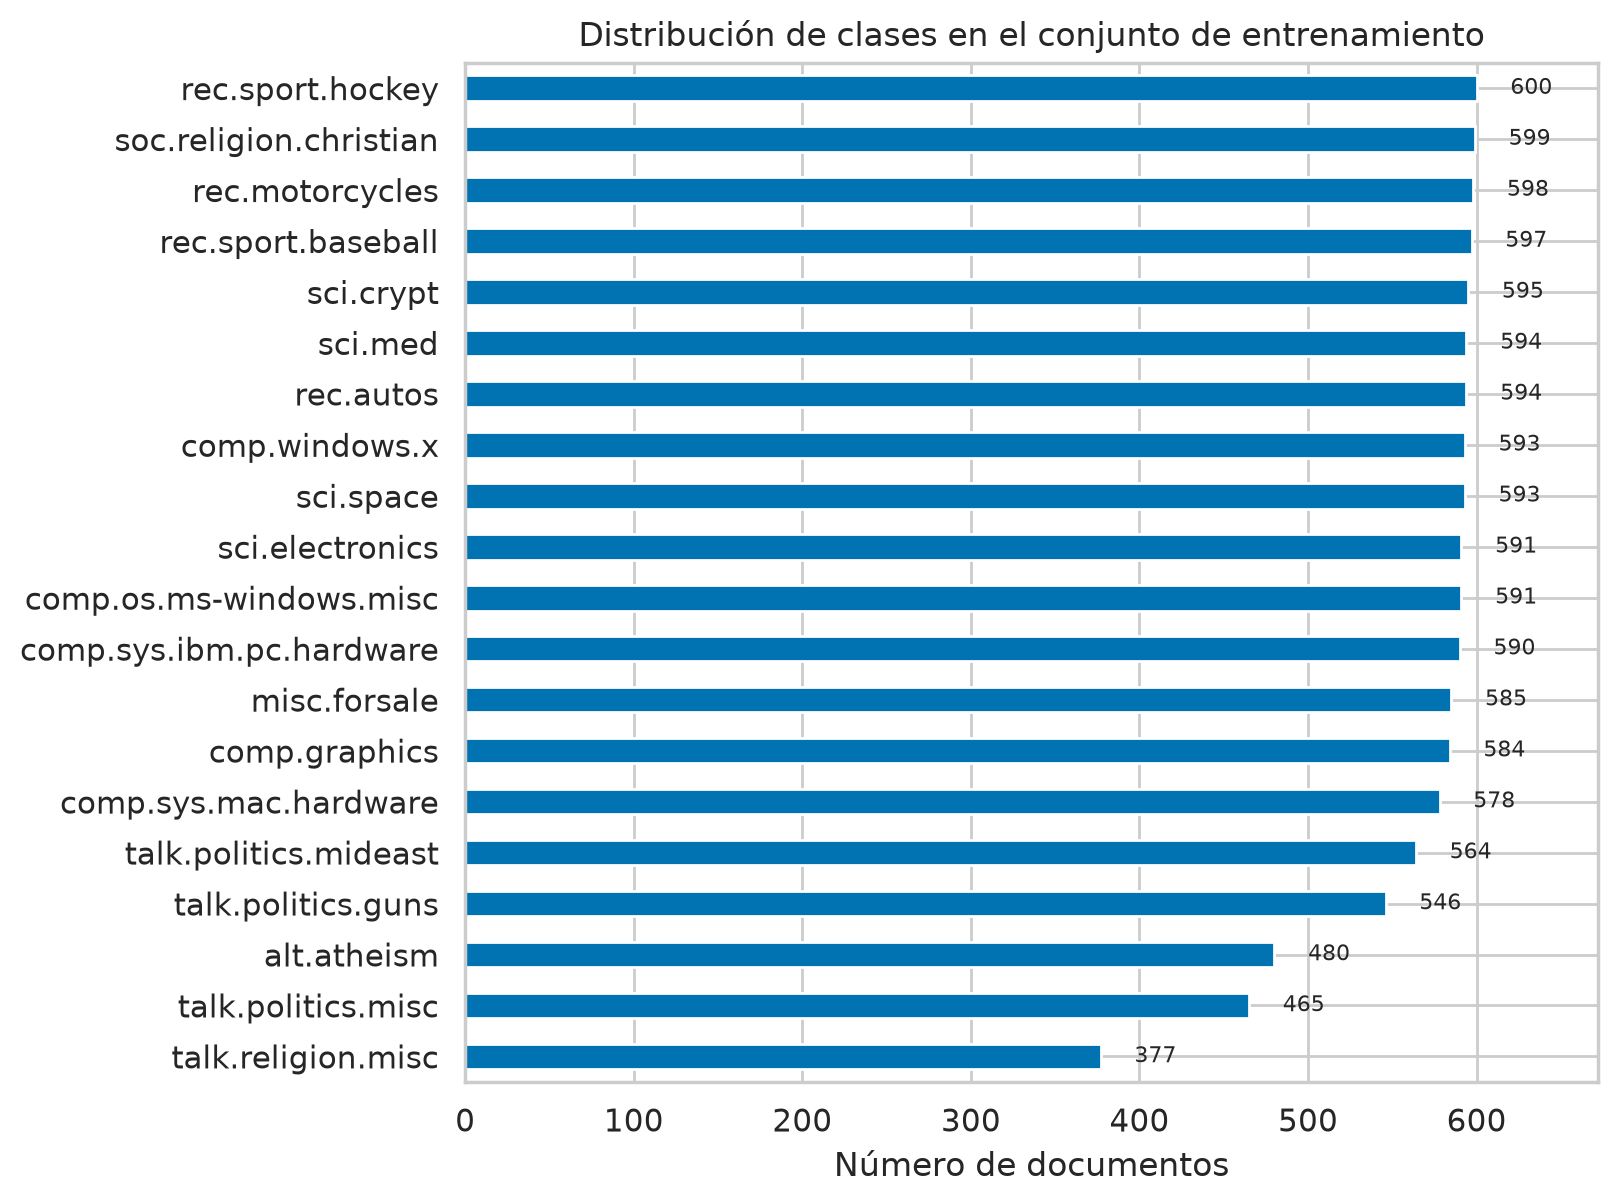
\includegraphics[width=0.78\textwidth]{eda_distribucion_clases.png}
  \caption{Distribución de las 20 clases en el conjunto de entrenamiento.}
  \label{fig:clases}
\end{figure}

\subsection{Preprocesamiento}

El preprocesamiento se implementa en \texttt{src/data.py} y comprende:
\begin{enumerate}[leftmargin=1.2em]
  \item \textbf{Eliminación de metadatos.} Se descartan cabeceras, pies de página y citas con la opción \texttt{remove=('headers','footers','quotes')} de scikit-learn. Sin este paso, campos como \texttt{Newsgroups:} o \texttt{Path:} contienen la etiqueta y producen una fuga de información severa.
  \item \textbf{Texto crudo como entrada.} No se eliminan \textit{stopwords} ni se aplica stemming; la capa \texttt{TextVectorization} pasa el texto a minúsculas, elimina puntuación y tokeniza por espacios.
  \item \textbf{Vocabulario aprendido solo en entrenamiento.} El vectorizador se adapta con el conjunto de entrenamiento; validación y prueba se transforman con ese vocabulario. Esto evita que las estadísticas del test influyan en el modelo.
  \item \textbf{Partición estratificada.} El 10\,\% del entrenamiento oficial se reserva para validación (\NVal{} documentos) y el 90\,\% restante (\NTrain{} documentos) se usa para ajustar los pesos. El conjunto de prueba oficial (\NTest{} documentos) se utiliza una sola vez, al final.
\end{enumerate}

La Figura~\ref{fig:longitudes} muestra que la mayoría de los documentos son cortos (mediana de \WordsMedian{} palabras), pero existen colas largas de hasta \WordsMax{} palabras. Como TF-IDF no impone una longitud fija, los documentos largos no se truncan; esto es una diferencia importante frente a las RNN de la segunda entrega, que requieren secuencias de longitud acotada.

Un hallazgo del preprocesamiento es que \EmptyDocs{} documentos del conjunto de entrenamiento quedan sin palabras después de eliminar cabeceras, pies y citas. Corresponden a mensajes cuyo contenido era únicamente metadatos o texto citado. Estos documentos se conservan para no alterar la partición oficial, pero son intrínsecamente inclasificables: el modelo recibe un vector TF-IDF nulo y predice la clase prioritaria. En el conjunto de prueba representan una fracción similar y establecen un techo práctico a la exactitud alcanzable.

\begin{figure}[H]
  \centering
  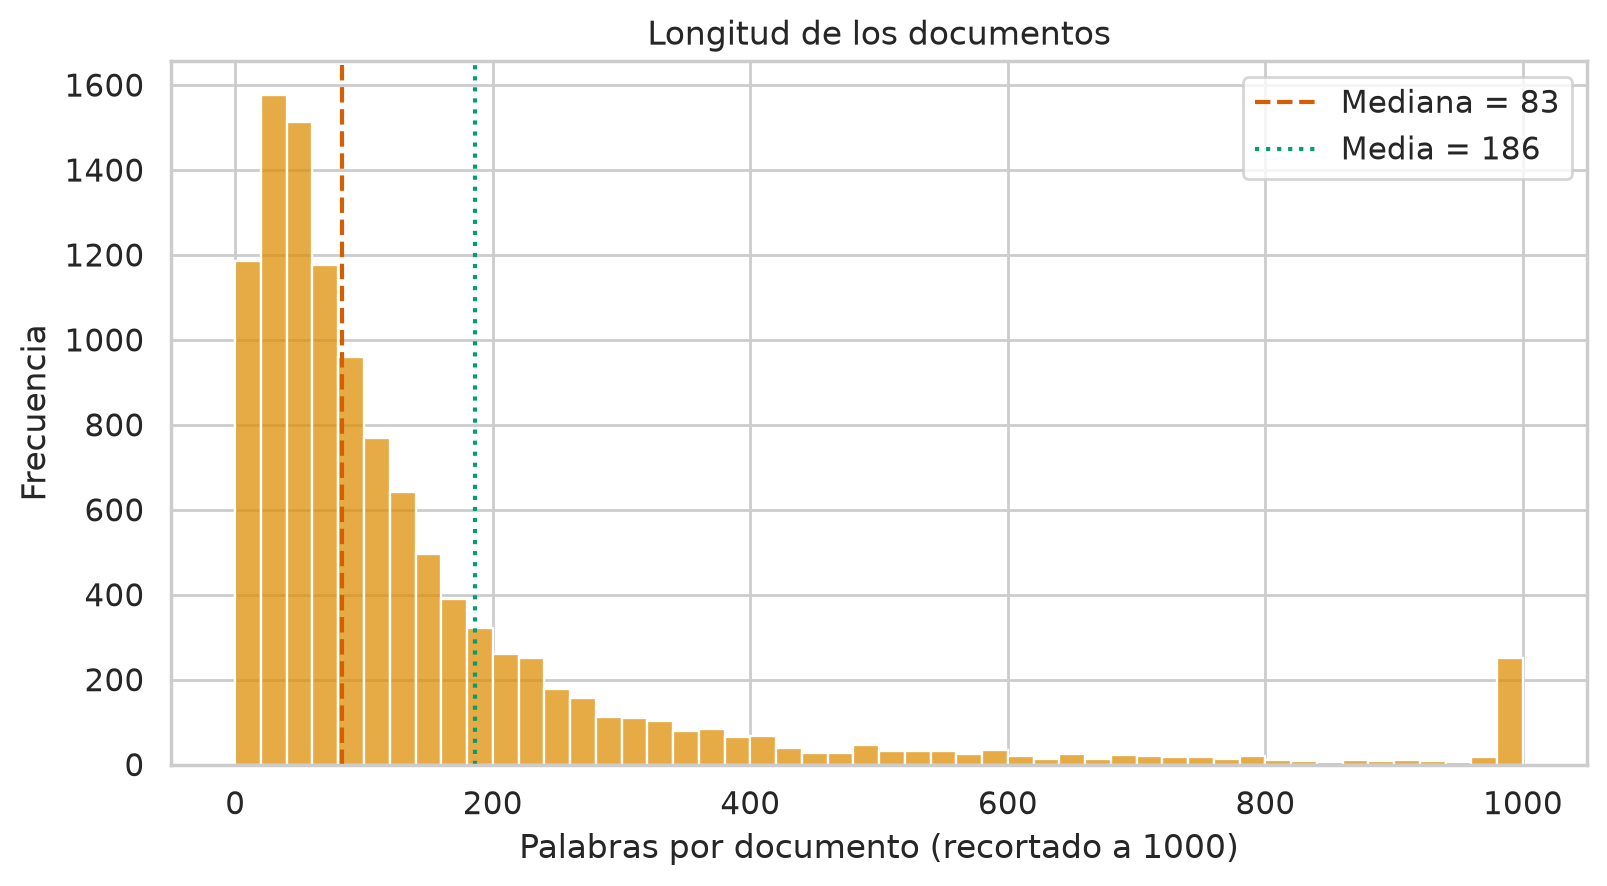
\includegraphics[width=0.78\textwidth]{eda_longitud_documentos.png}
  \caption{Distribución de la longitud de los documentos (recortada a 1000 palabras para visualización).}
  \label{fig:longitudes}
\end{figure}

\subsection{Análisis exploratorio}

Además de la distribución de clases, se observó que muchos mensajes son respuestas dentro de un hilo y comparten vocabulario con otros grupos. Por ejemplo, mensajes de \texttt{comp.os.ms-windows.misc} discuten hardware y mensajes de \texttt{talk.politics.misc} discuten religión. Esta cercanía semántica anticipa las confusiones que se analizan en la Sección~\ref{sec:resultados}.

% ======================================================================
\section{Arquitectura de la red}\label{sec:arquitectura}
% ======================================================================

La arquitectura es una MLP que recibe texto y produce una distribución sobre 20 clases. La Figura~\ref{fig:arquitectura} resume el flujo y la Tabla~\ref{tab:capas} detalla las dimensiones y el número de parámetros.

\begin{figure}[H]
\centering
\begin{tikzpicture}[
  node distance=0.75cm and 0.65cm,
  box/.style={draw=uvblue, fill=uvlight, rounded corners=3pt, align=center,
              minimum height=1.05cm, minimum width=2.05cm, font=\small},
  arrow/.style={-{Latex[length=2.2mm]}, thick, draw=uvgray}
]
  \node[box] (texto) {Texto\\crudo};
  \node[box, right=of texto] (tfidf) {TF-IDF\\\Vocab{} términos};
  \node[box, right=of tfidf] (d1) {Dense 256\\ReLU\\Dropout 0.3};
  \node[box, right=of d1] (out) {Softmax\\20 clases};
  \draw[arrow] (texto) -- (tfidf);
  \draw[arrow] (tfidf) -- (d1);
  \draw[arrow] (d1) -- (out);
\end{tikzpicture}
\caption{Arquitectura del Perceptrón Multicapa. La capa \texttt{TextVectorization} no tiene parámetros entrenables; aprende el vocabulario y calcula TF-IDF.}
\label{fig:arquitectura}
\end{figure}

\begin{table}[H]
\centering
\caption{Resumen de capas y parámetros del modelo principal.}
\label{tab:capas}
\begin{tabular}{lccc}
\toprule
Capa & Salida & Activación & Parámetros \\
\midrule
\texttt{TextVectorization} (TF-IDF) & 20.000 & --- & 0 \\
\texttt{Dense 1} & 256 & ReLU & 5.120.256 \\
\texttt{Dropout 1} & 256 & --- & 0 \\
\texttt{Dense de salida} & 20 & Softmax & 5.140 \\
\midrule
\textbf{Total} & & & \textbf{\ParamsExact} \\
\bottomrule
\end{tabular}
\end{table}

\subsection{Decisiones de diseño}

\textbf{Entrada TF-IDF en lugar de embeddings.} Una alternativa habitual es aprender embeddings de palabras y promediarlos o concatenarlos. Sin embargo, para una MLP pura sobre un corpus pequeño, TF-IDF ofrece una señal densa y bien regularizada, entrena en segundos y sirve como línea base reproducible. Los embeddings sin contexto pierden gran parte de la información y requieren muchos más datos para ajustarse; se explorarán en la Entrega 2 con arquitecturas secuenciales.

\textbf{Una capa oculta de 256 neuronas.} Esta capa aprende combinaciones lineales de términos y es suficiente para un problema con 20 clases y \NTrain{} ejemplos. El barrido de hiperparámetros (Sección~\ref{sec:resultados}) mostró que añadir una segunda capa (512--256) reduce el F1 macro de \MacroF{} a \TwoLayerF{} y que una tercera capa lo reduce a \DeepF{}; es decir, la capacidad adicional se dedica a memorizar el entrenamiento y no a generalizar. Se eligió por tanto la configuración más simple que obtuvo el mejor resultado.

\textbf{Dropout.} Se aplica una tasa de 0.3 después de la capa oculta, que concentra 5.1 millones de parámetros y por tanto el mayor riesgo de sobreajuste. La comparación con una tasa mayor (0.5--0.4) y con regularización L2 se presenta en la Sección~\ref{sec:resultados}.

\textbf{Salida softmax y pérdida.} Al ser clasificación multiclase mutuamente excluyente, se usa una neurona por clase con softmax y entropía cruzada categórica dispersa (\texttt{sparse\_categorical\_crossentropy}), que evita convertir las etiquetas a vectores one-hot.

% ======================================================================
\section{Entrenamiento y ajuste de parámetros}\label{sec:entrenamiento}
% ======================================================================

\subsection{Protocolo}

Todos los experimentos comparten la misma partición, semilla (42), vocabulario adaptado solo en entrenamiento y criterio de parada temprana, de modo que las diferencias se puedan atribuir a la configuración evaluada. La Tabla~\ref{tab:condiciones} resume las condiciones.

\begin{table}[H]
\centering
\caption{Condiciones de entrenamiento del modelo principal.}
\label{tab:condiciones}
\begin{tabular}{ll}
\toprule
Elemento & Valor \\
\midrule
Entrada & Texto crudo (sin cabeceras, pies ni citas) \\
Representación & TF-IDF, vocabulario de \Vocab{} términos \\
Optimizador & Adam, $\eta = 10^{-3}$ \\
Pérdida & Entropía cruzada categórica dispersa \\
Batch & 128 \\
Épocas máximas & 25 \\
Parada temprana & \texttt{val\_accuracy}, paciencia 5, $\Delta_{\min}=10^{-4}$ \\
Regularización & Dropout 0.3 \\
Semilla & 42 (determinismo activado) \\
Software & TensorFlow 2.20, Keras 3.15, scikit-learn 1.7, Python 3.12 \\
Hardware & CPU Intel Core i5-9400F, 6 núcleos, 31 GB RAM \\
\bottomrule
\end{tabular}
\end{table}

Se eligió la exactitud de validación como criterio de parada en lugar de la pérdida porque, en experimentos preliminares, la pérdida de validación aumentaba por sobreconfianza mientras la exactitud seguía mejorando. La parada temprana restaura los pesos de la mejor época, y el conjunto de prueba se evalúa una única vez con esos pesos.

\subsection{Espacio de búsqueda}

Se evaluaron \NumExperiments{} configuraciones:
\begin{itemize}[leftmargin=1.2em]
  \item \textbf{Profundidad:} modelo lineal sin capas ocultas (regresión softmax sobre TF-IDF), una capa de 256 (principal), dos capas de 512--256 y tres capas de 512--256--128.
  \item \textbf{Regularización:} dropout 0.3 (principal), dropout 0.5--0.4 y L2 de $10^{-4}$ sobre los kernels.
  \item \textbf{Vocabulario:} \Vocab{} y 10.000 términos.
  \item \textbf{Balanceo:} pesos de clase inversamente proporcionales a su frecuencia.
  \item \textbf{Tasa de aprendizaje:} $10^{-3}$ y $5\times10^{-4}$.
\end{itemize}

La Tabla~\ref{tab:experimentos} presenta los resultados en el conjunto de prueba, ordenados por F1 macro. La Figura~\ref{fig:comparacion} los compara visualmente.

\begin{table}[H]
\centering
\caption{Resultados de las configuraciones evaluadas en el conjunto de prueba, ordenadas por F1 macro.}
\label{tab:experimentos}
\footnotesize
\setlength{\tabcolsep}{3pt}
\begin{tabular}{lccccccccc}
\toprule
Configuración & Capas & Drop. & Vocab. & Bal. & Parám. & Ép. & Exact. & F1 & Top-3 \\
\midrule
\textbf{MLP 1$\times$256 (principal)} & 256 & 0.3 & 20k & No & 5.1M & 8 & 0.6771 & 0.6663 & 0.8452 \\
MLP 2$\times$512--256, lr 5e-4 & 512-256 & 0.4-0.3 & 20k & No & 10.4M & 10 & 0.6741 & 0.6653 & 0.8376 \\
MLP 2$\times$512--256 & 512-256 & 0.4-0.3 & 20k & No & 10.4M & 10 & 0.6680 & 0.6578 & 0.8240 \\
MLP 2$\times$512--256, balanceado & 512-256 & 0.4-0.3 & 20k & Sí & 10.4M & 8 & 0.6686 & 0.6568 & 0.8258 \\
MLP 2$\times$512--256, dropout 0.5--0.4 & 512-256 & 0.5-0.4 & 20k & No & 10.4M & 9 & 0.6644 & 0.6566 & 0.8266 \\
Lineal (sin capas ocultas) & --- & - & 20k & No & 0.4M & 11 & 0.6572 & 0.6451 & 0.8368 \\
MLP 3$\times$512--256--128 & 512-256-128 & 0.4-0.3-0.2 & 20k & No & 10.4M & 13 & 0.6498 & 0.6433 & 0.8140 \\
MLP 2$\times$512--256, L2 1e-4 & 512-256 & 0.4-0.3 & 20k & No & 10.4M & 12 & 0.6455 & 0.6393 & 0.8177 \\
MLP 2$\times$512--256, vocab. 10k & 512-256 & 0.4-0.3 & 10k & No & 5.3M & 11 & 0.6439 & 0.6358 & 0.8123 \\
\bottomrule
\end{tabular}
\end{table}


\begin{figure}[H]
  \centering
  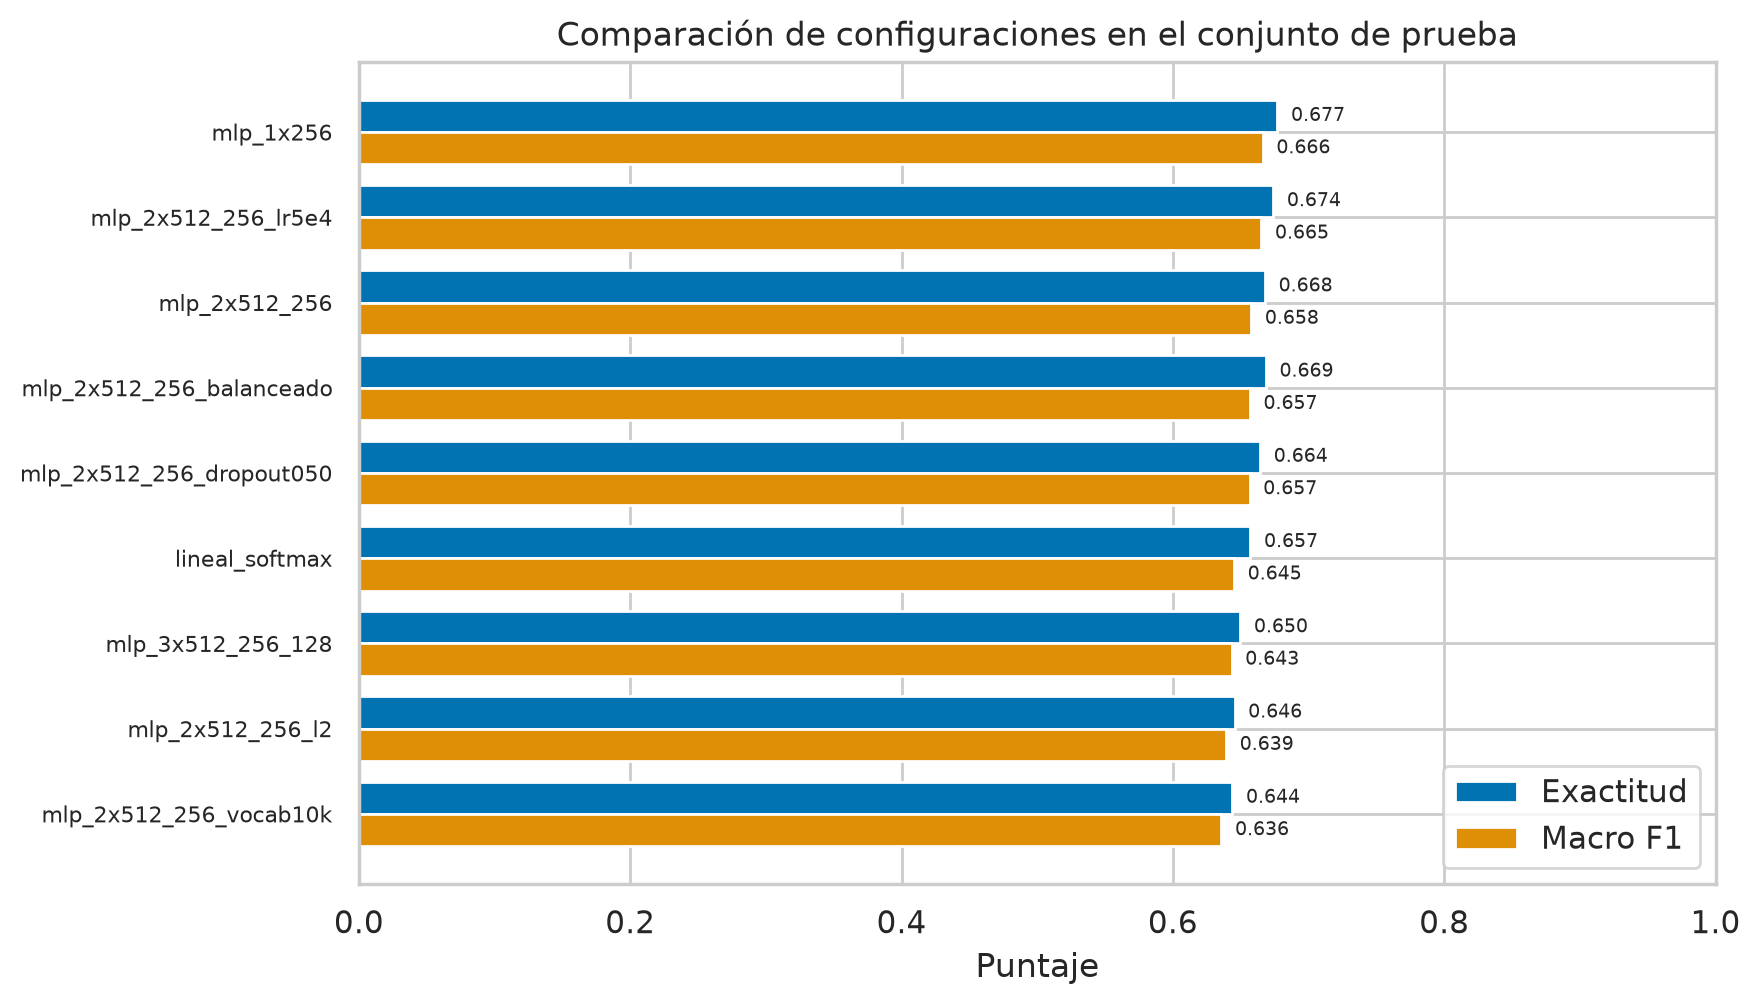
\includegraphics[width=0.9\textwidth]{comparacion_experimentos.png}
  \caption{Exactitud y F1 macro en prueba para las configuraciones evaluadas.}
  \label{fig:comparacion}
\end{figure}

\subsection{Costo computacional}

El modelo principal tiene \NumParams{} millones de parámetros y se entrenó en alrededor de 30 segundos en CPU (sin GPU), incluyendo la adaptación del vocabulario. La mayor parte del costo corresponde a la capa densa, que multiplica un vector TF-IDF de \Vocab{} dimensiones por una matriz de $20.000\times256$. Este costo es aceptable para un corpus de este tamaño y permite iterar rápidamente sobre hiperparámetros.

% ======================================================================
\section{Resultados y análisis}\label{sec:resultados}
% ======================================================================

\subsection{Desempeño del modelo principal}

La Tabla~\ref{tab:metricas} reporta las métricas del modelo principal en el conjunto de prueba. El modelo se entrenó durante \EpochsRun{} épocas y la mejor época fue la \BestEpoch{}, con una exactitud de validación de \BestValAcc{}.

\begin{table}[H]
\centering
\caption{Métricas del modelo principal en el conjunto de prueba (\NTest{} documentos).}
\label{tab:metricas}
\begin{tabular}{lc}
\toprule
Métrica & Valor \\
\midrule
Exactitud & \Accuracy \\
Precisión macro & \MacroPrecision \\
Recall macro & \MacroRecall \\
F1 macro & \MacroF \\
F1 ponderado & \WeightedF \\
Exactitud top-3 & \TopThree \\
\bottomrule
\end{tabular}
\end{table}

La exactitud de \Accuracy{} es muy superior al azar (5\,\% para 20 clases balanceadas) y al \emph{baseline} lineal, que obtiene \LinearAcc{}. La exactitud top-3 de \TopThree{} indica que, en más de tres de cada cuatro documentos, la clase correcta está entre las tres más probables; esto es relevante en aplicaciones donde un humano revisa las sugerencias del modelo.

La brecha entre la exactitud de validación (\BestValAcc{}) y la de prueba (\Accuracy{}) es de \ValTestGap{} puntos porcentuales. Parte de esta diferencia se explica por el tamaño reducido de la validación (\NVal{} documentos), que produce una estimación con alta varianza, y parte por el sobreajuste del modelo a los documentos de entrenamiento. Además, la distribución de longitudes y de grupos no es idéntica entre las particiones: el conjunto de prueba contiene mensajes de fechas y hilos distintos. La Figura~\ref{fig:curvas} muestra la evolución típica: la exactitud de entrenamiento supera el 95\,\%, mientras la de validación se estabiliza entre el 72\,\% y el 75\,\%.

\begin{figure}[H]
  \centering
  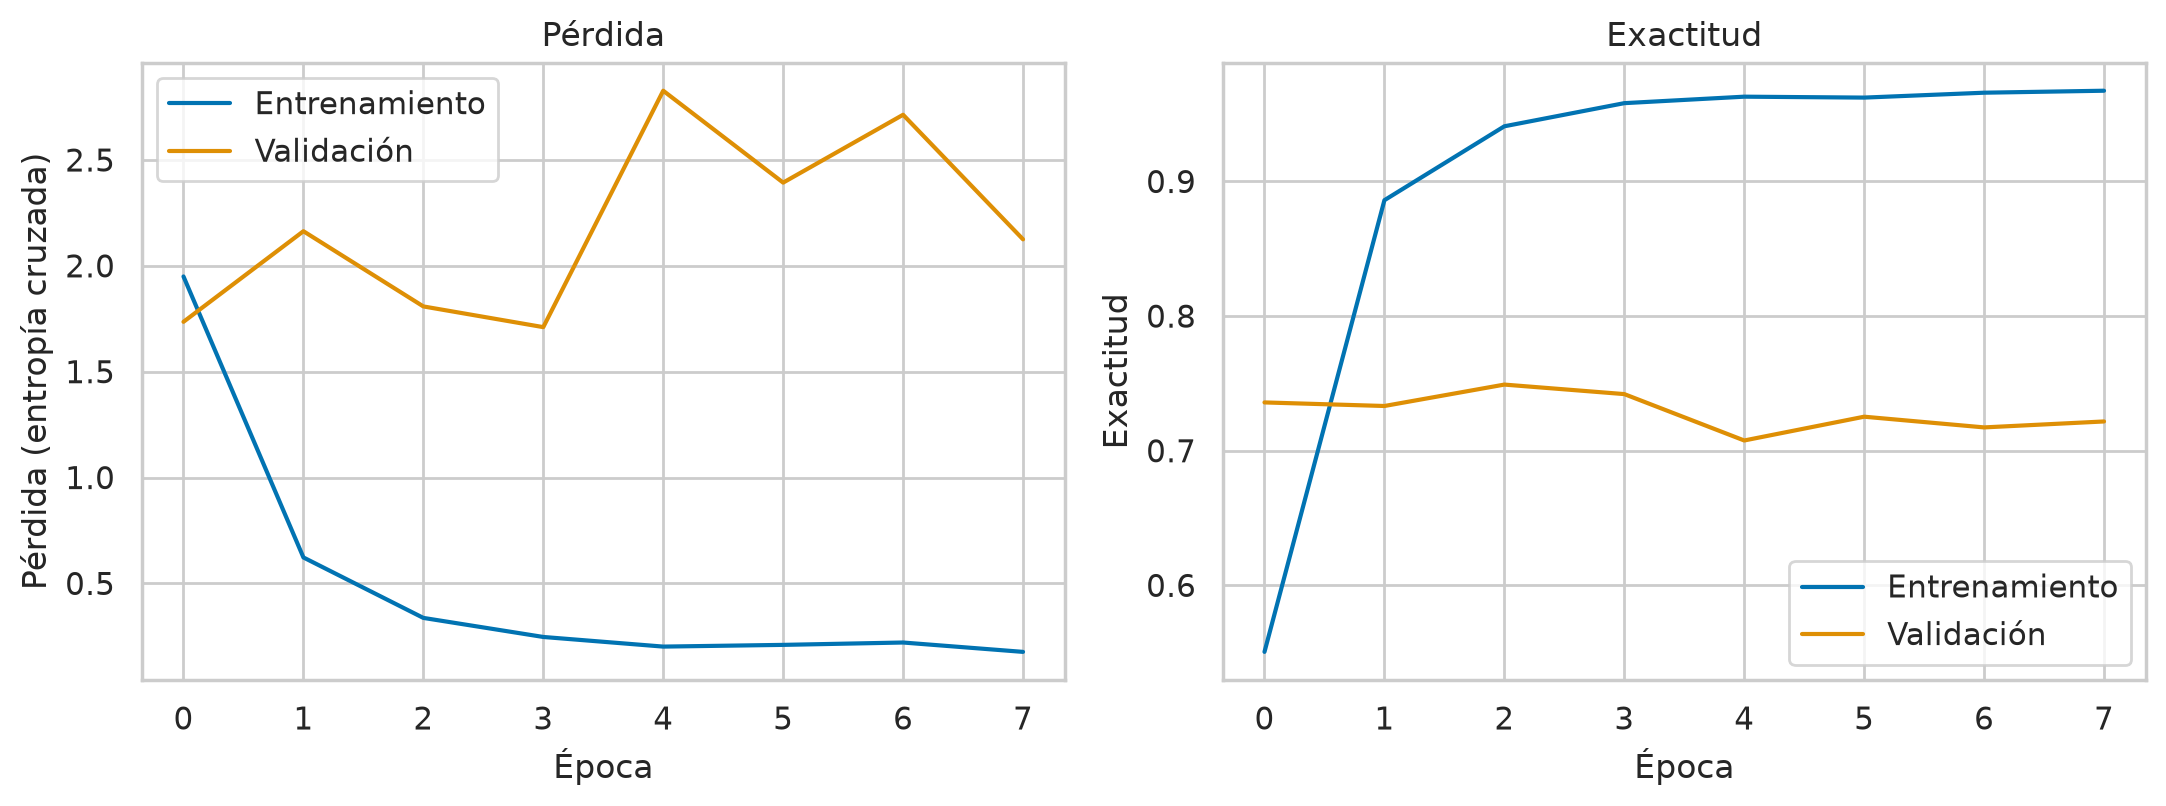
\includegraphics[width=\textwidth]{curvas_entrenamiento_primary.png}
  \caption{Curvas de pérdida y exactitud del modelo principal. La parada temprana restaura los pesos de la mejor época de validación.}
  \label{fig:curvas}
\end{figure}

\subsection{Análisis por clase}

La Figura~\ref{fig:f1clase} y la Tabla~\ref{tab:por-clase} (Apéndice~\ref{ap:repro}) muestran un desempeño heterogéneo. Las clases con mayor F1 son \texttt{rec.sport.hockey}, \texttt{comp.windows.x} y \texttt{misc.forsale}; las más difíciles son \texttt{talk.religion.misc}, \texttt{alt.atheism} y \texttt{talk.politics.misc}. Estas últimas son también las de menor soporte o las que comparten vocabulario con varias clases.

\begin{figure}[H]
  \centering
  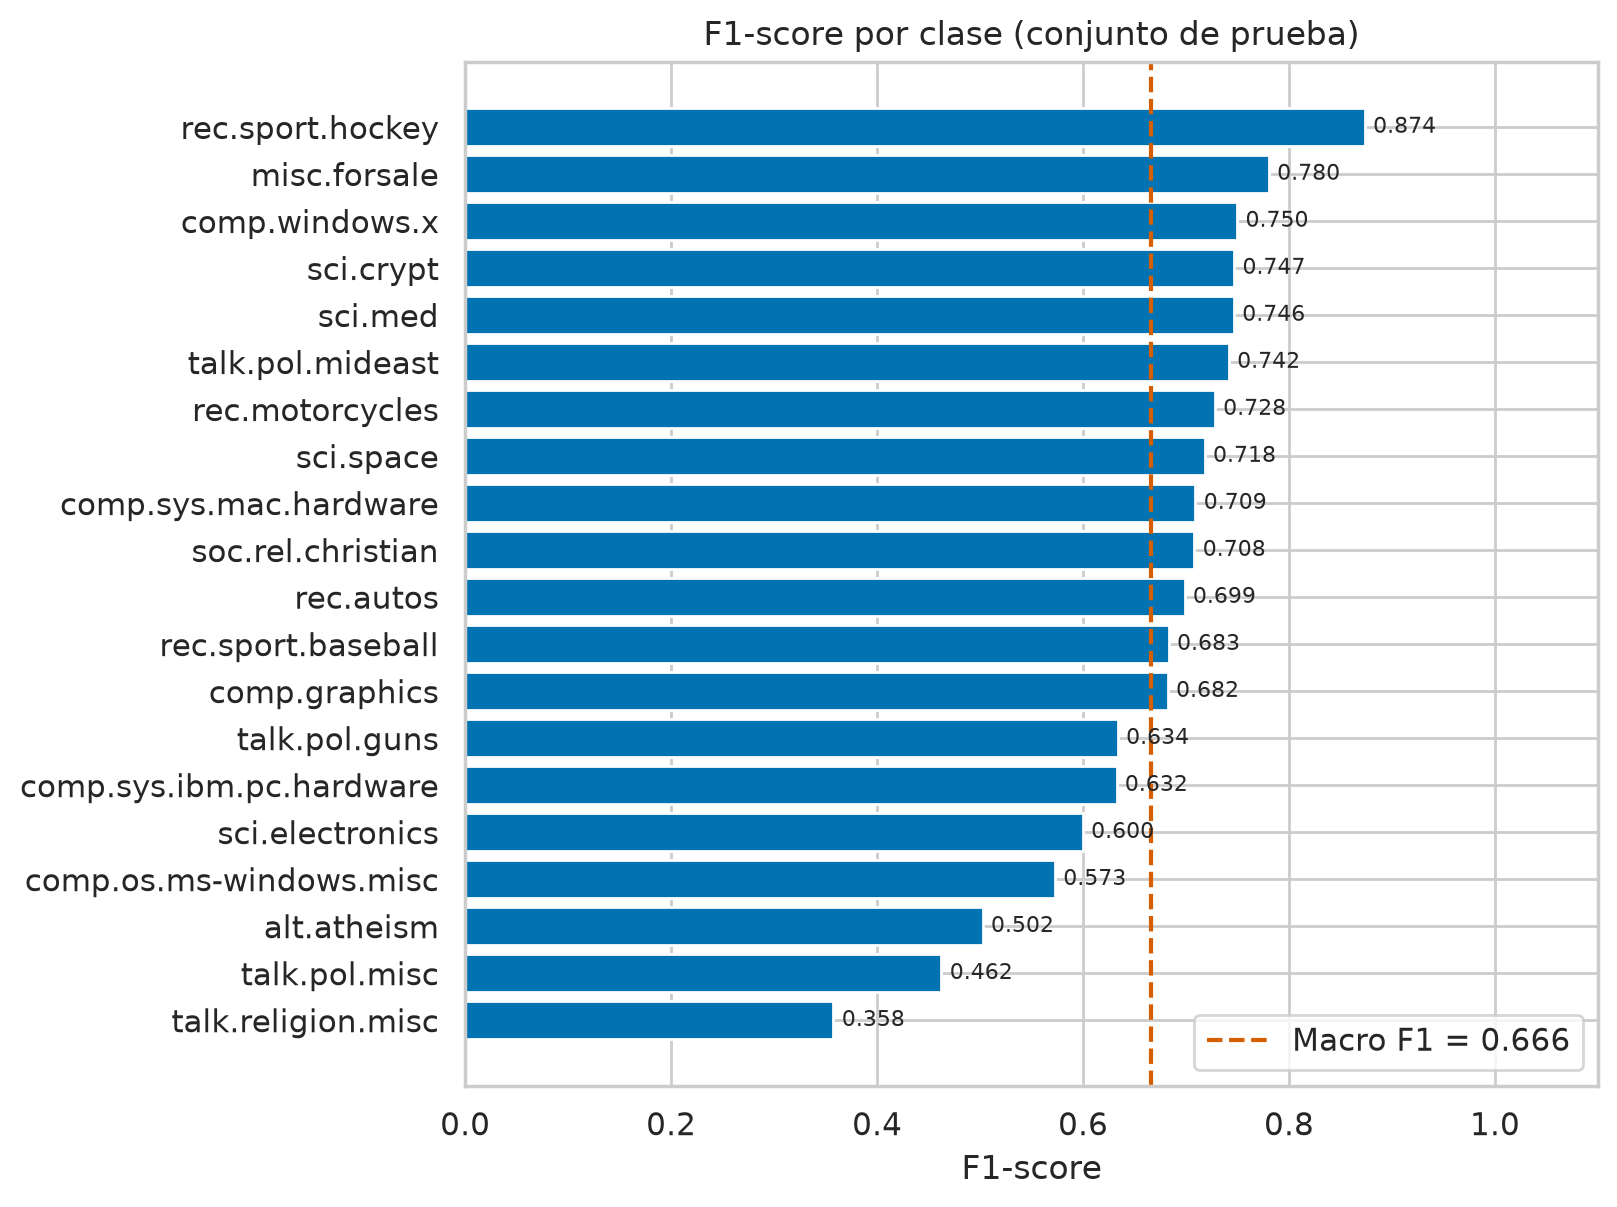
\includegraphics[width=0.82\textwidth]{f1_por_clase_primary.png}
  \caption{F1-score por clase en el conjunto de prueba.}
  \label{fig:f1clase}
\end{figure}

\subsection{Matriz de confusión y errores}

La Figura~\ref{fig:matriz} presenta la matriz de confusión normalizada por clase real. La diagonal concentra la mayor parte de la masa, pero se observan bloques fuera de ella:
\begin{itemize}[leftmargin=1.2em]
  \raggedright
  \item \textbf{Computación:} \texttt{comp.os.ms-windows.misc}, \texttt{comp.sys.ibm.pc.hardware} y \texttt{comp.sys.mac.hardware} se confunden entre sí porque comparten términos de hardware, sistemas operativos y controladores.
  \item \textbf{Religión:} \texttt{alt.atheism}, \texttt{soc.religion.christian} y \texttt{talk.religion.misc} comparten vocabulario y argumentos; además, los hilos de discusión mezclan las tres perspectivas.
  \item \textbf{Política:} \texttt{talk.politics.guns}, \texttt{talk.politics.mideast} y \texttt{talk.politics.misc} presentan solapamiento temático y de entidades nombradas.
\end{itemize}

\begin{figure}[H]
  \centering
  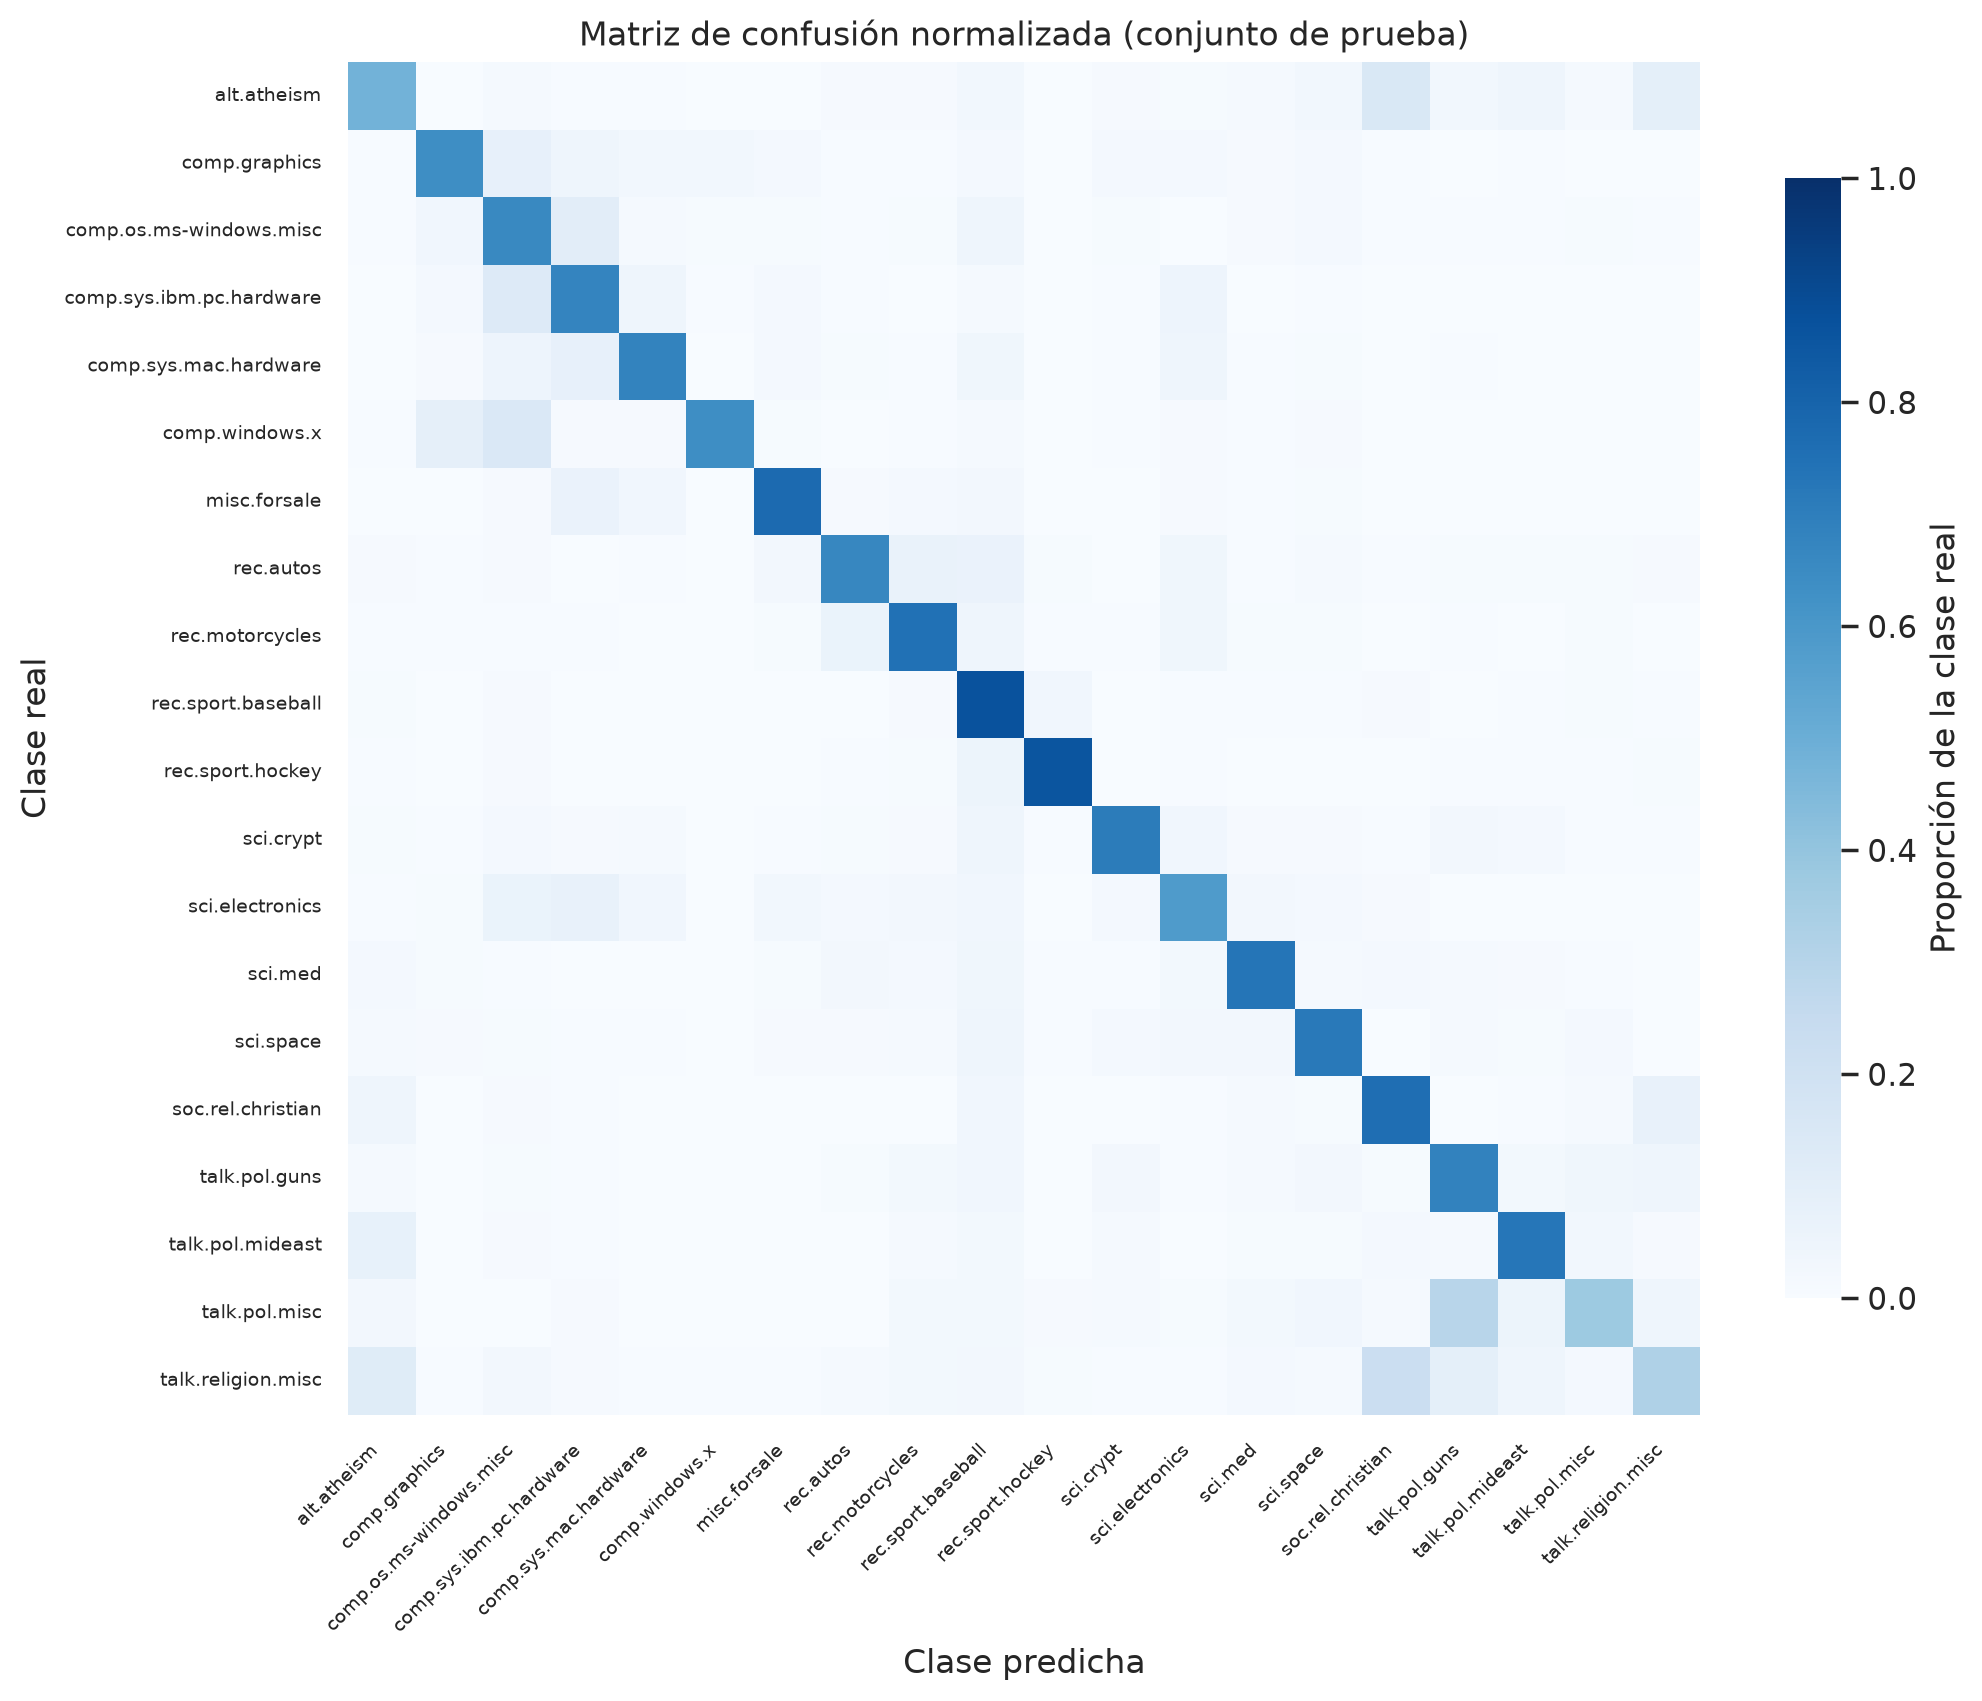
\includegraphics[width=0.86\textwidth]{matriz_confusion_primary.png}
  \caption{Matriz de confusión normalizada por clase real del modelo principal.}
  \label{fig:matriz}
\end{figure}

\begin{table}[H]
\centering
\caption{Confusiones más frecuentes del modelo principal.}
\label{tab:confusiones}
\small
\begin{tabular}{llcc}
\toprule
Clase real & Clase predicha & Casos & \% de la clase real \\
\midrule
talk.politics.misc & talk.politics.guns & 91 & 29.4\% \\
comp.windows.x & comp.os.ms-windows.misc & 58 & 14.7\% \\
talk.religion.misc & soc.religion.christian & 56 & 22.3\% \\
comp.sys.ibm.pc.hardware & comp.os.ms-windows.misc & 52 & 13.3\% \\
alt.atheism & soc.religion.christian & 48 & 15.0\% \\
comp.os.ms-windows.misc & comp.sys.ibm.pc.hardware & 42 & 10.7\% \\
comp.windows.x & comp.graphics & 36 & 9.1\% \\
comp.graphics & comp.os.ms-windows.misc & 33 & 8.5\% \\
\bottomrule
\end{tabular}
\end{table}


Un análisis cualitativo de los errores muestra que muchos documentos mal clasificados son cortos, con pocas palabras discriminativas, o son respuestas que citan el mensaje anterior y comparten su vocabulario. TF-IDF no distingue el tema principal del documento de las palabras citadas, lo que sugiere que un modelo secuencial podría mejorar al modelar el orden y el contexto.

\subsection{Efecto de los hiperparámetros}

\textbf{Profundidad.} El modelo lineal sin capas ocultas obtiene \LinearAcc{} de exactitud y \LinearF{} de F1 macro. Una capa de 256 neuronas (modelo principal) mejora a \Accuracy{} y \MacroF{}. Añadir una segunda capa (512--256) baja a \TwoLayerAcc{} y \TwoLayerF{}, y una tercera capa (512--256--128) baja a \DeepAcc{} y \DeepF{}. La ganancia proviene de la primera capa oculta; la capacidad adicional de las redes más profundas se dedica a memorizar el entrenamiento y no aporta información nueva.

\textbf{Dropout.} Aumentar el dropout a 0.5--0.4 en la red de dos capas produce \DropoutAcc{} de exactitud y \DropoutF{} de F1 macro, por debajo del modelo principal. Un dropout excesivo en la primera capa dificulta el aprendizaje de las combinaciones de términos, mientras que una tasa menor aumenta el sobreajuste; 0.3 resulta un compromiso razonable para una sola capa de 256 neuronas.

\textbf{Vocabulario.} Reducir el vocabulario a 10.000 términos reduce la exactitud a \VocabTenAcc{} y el F1 macro a \VocabTenF{}. El corpus contiene muchos términos técnicos y nombres propios poco frecuentes que son informativos; truncar el vocabulario los convierte en \texttt{[UNK]} y elimina señal.

\textbf{Balanceo de clases.} Los pesos balanceados producen \BalancedAcc{} de exactitud y \BalancedF{} de F1 macro. El F1 macro no supera al del modelo sin balanceo, lo que sugiere que el desbalance del corpus no es lo bastante severo para justificar el costo de reponderar las clases.

\textbf{Tasa de aprendizaje y L2.} La tasa $5\times10^{-4}$ obtiene \LrAcc{} y \LrF{}, y L2 $10^{-4}$ obtiene \LtwoAcc{} y \LtwoF{}. Ninguna supera al modelo principal: una tasa menor requiere más épocas y L2 compite con el dropout sin aportar una mejora clara.

\begin{figure}[H]
  \centering
  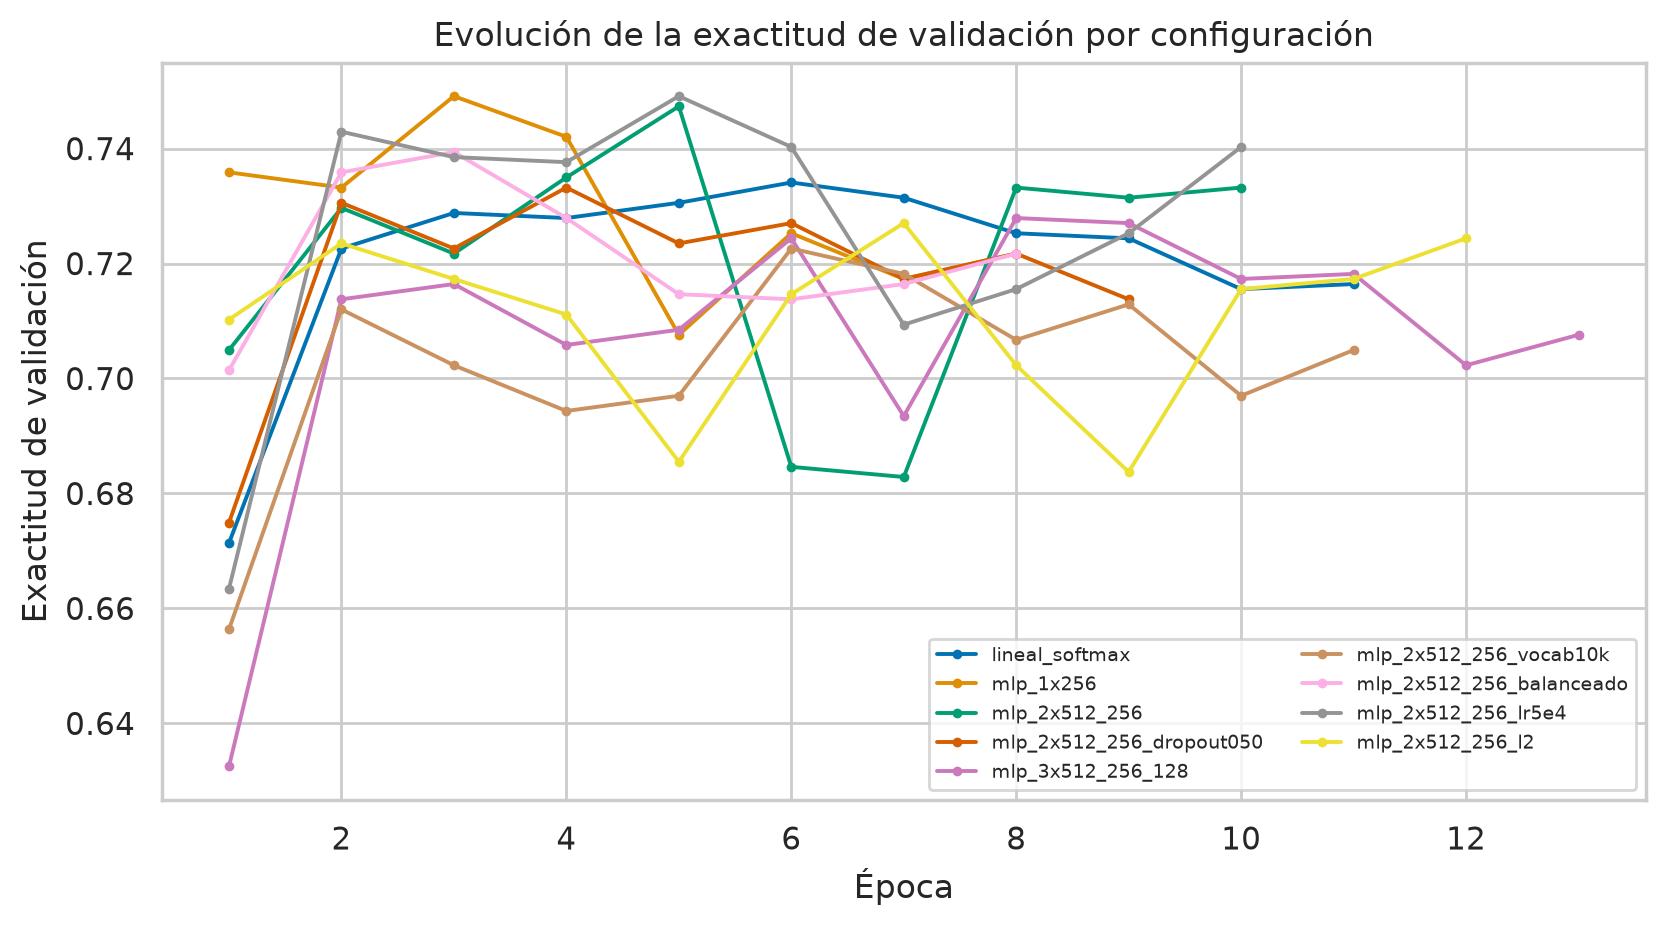
\includegraphics[width=0.9\textwidth]{curvas_validacion_experimentos.png}
  \caption{Exactitud de validación por época para las configuraciones evaluadas.}
  \label{fig:valcurves}
\end{figure}

\subsection{Discusión}

Los resultados son coherentes con la literatura: los modelos lineales sobre TF-IDF son líneas base fuertes en 20 Newsgroups, y las redes neuronales aportan mejoras moderadas cuando se controla el sobreajuste \cite{joachims1998,lang1995}. La principal limitación de la arquitectura es que la representación \textit{bag-of-words} ignora el orden de las palabras y la estructura del discurso. Además, el vocabulario se aprende solo del entrenamiento y no incorpora conocimiento semántico externo (por ejemplo, embeddings preentrenados). A esto se suman los \EmptyDocs{} documentos de entrenamiento que quedan vacíos tras eliminar metadatos y citas: son inclasificables y el modelo solo puede aprender de ellos la distribución prioritaria, lo que introduce ruido y reduce la exactitud máxima alcanzable.

Otra limitación metodológica es que la selección de hiperparámetros se hizo con un único split de validación de \NVal{} documentos y una sola semilla. Las diferencias de uno o dos puntos porcentuales entre configuraciones pueden estar dentro del ruido de estimación. Para la entrega final sería recomendable usar validación cruzada o varias semillas y reportar media y desviación estándar. También conviene repetir la evaluación con la métrica F1 macro como criterio principal de selección, tal como se hizo en este trabajo.

Finalmente, el desbalance de clases y las confusiones entre grupos temáticamente cercanos sugieren que parte del error es irreducible con bolsas de palabras: dos documentos pueden compartir casi todo el vocabulario y pertenecer a grupos distintos porque el grupo de noticias es una convención social, no un tema puro.

% ======================================================================
\section{Conclusiones}\label{sec:conclusiones}
% ======================================================================

Se construyó y evaluó una MLP en Keras/TensorFlow para clasificar 20 Newsgroups en 20 categorías. El modelo combina una representación TF-IDF de \Vocab{} términos con una capa densa de 256 neuronas, dropout 0.3 y salida softmax. En el conjunto de prueba obtuvo una exactitud de \Accuracy{}, un F1 macro de \MacroF{} y una exactitud top-3 de \TopThree{}, superando al azar y a un modelo lineal.

El ajuste de hiperparámetros mostró que una sola capa oculta es suficiente, que añadir capas reduce el F1 macro, que un vocabulario más pequeño pierde señal y que el balanceo de clases no compensa la pérdida de exactitud. El dropout 0.3 y el vocabulario completo ofrecen el mejor compromiso. La brecha entre validación y prueba y el análisis de confusiones evidencian sobreajuste y solapamiento semántico entre clases.

Como trabajo futuro para la Entrega 2, se propone reemplazar la representación TF-IDF por secuencias de tokens y comparar una RNN sin memoria (por ejemplo, una red densa sobre embeddings o una RNN simple) con una RNN con memoria (LSTM/GRU) o un Transformer. Estas arquitecturas pueden modelar el orden, el contexto y las dependencias de largo plazo que TF-IDF ignora, y se espera que mejoren especialmente en las clases con mayor confusión.

% ======================================================================
\begin{thebibliography}{9}
% ======================================================================

\bibitem{lang1995}
K. Lang, ``NewsWeeder: Learning to Filter Netnews,'' in \textit{Proceedings of the 12th International Conference on Machine Learning (ICML)}, 1995, pp. 331--339.

\bibitem{joachims1998}
T. Joachims, ``Text Categorization with Support Vector Machines: Learning with Many Relevant Features,'' in \textit{Proceedings of the 10th European Conference on Machine Learning (ECML)}, 1998, pp. 137--142.

\bibitem{rumelhart1986}
D. E. Rumelhart, G. E. Hinton, and R. J. Williams, ``Learning Representations by Back-Propagating Errors,'' \textit{Nature}, vol. 323, no. 6088, pp. 533--536, 1986.

\bibitem{kingma2015}
D. P. Kingma and J. Ba, ``Adam: A Method for Stochastic Optimization,'' in \textit{International Conference on Learning Representations (ICLR)}, 2015.

\bibitem{srivastava2014}
N. Srivastava, G. Hinton, A. Krizhevsky, I. Sutskever, and R. Salakhutdinov, ``Dropout: A Simple Way to Prevent Neural Networks from Overfitting,'' \textit{Journal of Machine Learning Research}, vol. 15, no. 1, pp. 1929--1958, 2014.

\bibitem{pedregosa2011}
F. Pedregosa \textit{et al.}, ``Scikit-learn: Machine Learning in Python,'' \textit{Journal of Machine Learning Research}, vol. 12, pp. 2825--2830, 2011.

\bibitem{tensorflow2016}
M. Abadi \textit{et al.}, ``TensorFlow: A System for Large-Scale Machine Learning,'' in \textit{12th USENIX Symposium on Operating Systems Design and Implementation (OSDI)}, 2016, pp. 265--283.

\end{thebibliography}

\newpage
\appendix
% ======================================================================
\section{Reproducibilidad y resultados por clase}\label{ap:repro}
% ======================================================================

\subsection*{Estructura del código}

\begin{verbatim}
Proyecto/
|-- src/
|   |-- config.py       # hiperparámetros y rutas
|   |-- data.py         # descarga, cacheo y partición
|   |-- model.py        # vectorizador TF-IDF y MLP
|   |-- train.py        # entrenamiento y evaluación
|   |-- experiments.py  # barrido de configuraciones
|   |-- plots.py        # figuras
|   |-- predict.py      # demo por línea de comandos
|   `-- build_docs.py   # tablas y macros del informe
|-- notebooks/
|   `-- entrega1_mlp.ipynb
|-- results/            # métricas, modelos y figuras
|-- informe/            # este documento
`-- presentacion/       # diapositivas
\end{verbatim}

\subsection*{Comandos}

\begin{verbatim}
uv venv --python 3.12 .venv
uv pip install --python .venv/bin/python -r requirements.txt

# Entrenar las 9 configuraciones y generar resultados
.venv/bin/python -m src.experiments

# Predicción interactiva
.venv/bin/python -m src.predict "texto a clasificar"

# Regenerar tablas y compilar el informe (requiere Tectonic instalado)
.venv/bin/python -m src.build_docs
tectonic -X compile informe/informe.tex
\end{verbatim}

\subsection*{Resultados por clase}

\begin{table}[H]
\centering
\caption{Métricas por clase del modelo principal en el conjunto de prueba.}
\label{tab:por-clase}
\small
\begin{tabular}{lcccc}
\toprule
Clase & Precisión & Recall & F1 & Soporte \\
\midrule
alt.atheism & 0.524 & 0.483 & 0.502 & 319 \\
comp.graphics & 0.730 & 0.640 & 0.682 & 389 \\
comp.os.ms-windows.misc & 0.506 & 0.660 & 0.573 & 394 \\
comp.sys.ibm.pc.hardware & 0.594 & 0.676 & 0.632 & 392 \\
comp.sys.mac.hardware & 0.740 & 0.681 & 0.709 & 385 \\
comp.windows.x & 0.904 & 0.641 & 0.750 & 395 \\
misc.forsale & 0.786 & 0.774 & 0.780 & 390 \\
rec.autos & 0.737 & 0.664 & 0.699 & 396 \\
rec.motorcycles & 0.711 & 0.746 & 0.728 & 398 \\
rec.sport.baseball & 0.563 & 0.869 & 0.683 & 397 \\
rec.sport.hockey & 0.891 & 0.857 & 0.874 & 399 \\
sci.crypt & 0.791 & 0.707 & 0.747 & 396 \\
sci.electronics & 0.615 & 0.585 & 0.600 & 393 \\
sci.med & 0.761 & 0.732 & 0.746 & 396 \\
sci.space & 0.715 & 0.721 & 0.718 & 394 \\
soc.religion.christian & 0.664 & 0.759 & 0.708 & 398 \\
talk.politics.guns & 0.588 & 0.687 & 0.634 & 364 \\
talk.politics.mideast & 0.755 & 0.729 & 0.742 & 376 \\
talk.politics.misc & 0.597 & 0.377 & 0.462 & 310 \\
talk.religion.misc & 0.401 & 0.323 & 0.358 & 251 \\
\midrule
Macro promedio & 0.679 & 0.666 & 0.666 & 7{,}532 \\
\bottomrule
\end{tabular}
\end{table}


\end{document}
